\chapter{Reporting}
For Varroa to fulfil a purpose, there needs to be an instance that reports the actions that have been executed.
Fo that reason there have to be entities that observe the parts of Varroa that execute the scenario.
Figure \ref{fig:ReportMapping} shows the entities that are responsible for observing the actions taken place as well as their hierarchy.

\section{Concept}
\begin{figure}[H]
	\begin{center}
		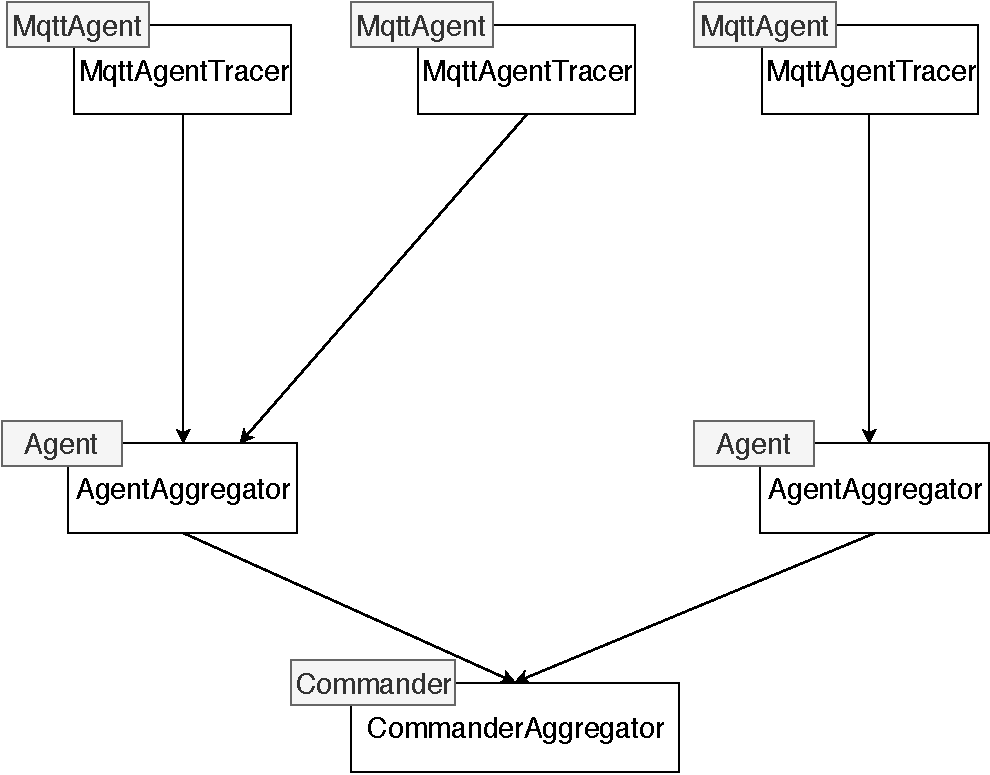
\includegraphics[scale=0.8]{Resources/PDF/ReportMapping}
		\caption{Reporting hierarchy}
		\label{fig:ReportMapping}
	\end{center}
\end{figure}




\subsection{Actions}

\subsection{Aggregation of Actions}

\section{Metrics}

\subsection{Time needed}

%TODO more different types of Metrics


